\section{Player module}

The library is a set of functions supporting communication with the game and creating tables and charts. These functions work in both Matlab and Octave environments.

\paragraph{SendData} \hspace{0pt} \\
Sending data to the server.

\begin{lstlisting}[style=Matlab-editor]
txt = SendData(IPAddressSend,portSend,data,name, args)
\end{lstlisting}

Description:
\begin{itemize}
\item  IPAddressSend -- server ip address,
\item  portSend -- server port,
\item  data -- data packet sent to the server,
\item  name  -- determines how the data is interpreted,
\item  args  -- arguments related to control information.
\end{itemize}

Returns the response from the server in xml format.

\paragraph{NumberToName} \hspace{0pt} \\
Replacing numbers representing field types with their names.
\begin{lstlisting}[style=Matlab-editor]
result = NumberToName(array, names)
\end{lstlisting}

Description:
\begin{itemize}
\item  array -- a table containing information about the map,
\item  names -- map field names.
\end{itemize}

Returns a table containing information about the map.

\paragraph{ChangeBeginEnd} \hspace{0pt} \\
Marking the beginnings and ends of paths.
\begin{lstlisting}[style=Matlab-editor]
result = ChangeBeginEnd(array)
\end{lstlisting}

Description:
\begin{itemize}
\item  array -- a table containing information about the map.
\end{itemize}

Returns a table containing information about the map.

\paragraph{TilemapToXML} \hspace{0pt} \\
Map conversion from an array to xml format.
\begin{lstlisting}[style=Matlab-editor]
txt = TilemapToXML(tilemap)
\end{lstlisting}

Description:
\begin{itemize}
\item  tilemap -- map in the form of an array.
\end{itemize}

Returns a map saved in xml format.

Example of sending a board creation command to the game:
\begin{lstlisting}[style=Matlab-editor]
%Server address
IPAddressSend = '127.0.0.1';
%Port on which the server is listening
portSend = 55001;
%Array representing the game board in which the numbers represent the types of tiles (1 - earth, 2 - water, which is an element of the opponents' path, 3 - the beginning of the path, 4 - the end of the path)
tilemap = [1	3	1	3	1	1	1	1	1	1	1	3	1	1	1 1;
           	1	2	1	2	1	1	1	1	1	1	1	2	1	1	1 1;
           	1	2	1	2	1	1	1	1	3	1	2	2	1	1	1 1;
           	1	2	1	2	1	1	1	1	2	1	2	1	1	1	1 1;
           	1	2	1	2	1	1	1	1	2	1	2	1	1	1	1 1;
           	1	2	1	2	2	1	1	1	2	1	2	2	1	1	1 1;
           	1	2	1	1	2	1	1	2	2	1	1	2	1	1	1 1;
           	1	2	1	2	2	1	1	2	1	1	2	2	1	1	1 1;
           	1	2	1	2	1	1	1	2	1	1	2	1	1	1	1 1;
           	1	2	1	2	1	1	1	2	2	1	2	2	2	2	1 1;
           	1	2	1	2	1	1	1	1	2	1	1	1	1	2	2 1;
           	1	2	1	2	2	1	1	1	2	2	4	1	1	1	2 1;
           	1	4	1	1	4	1	1	1	1	1	1	1	1	1	4 1];
%Tile type names. The position in the array corresponds to the number in the tilemap array
names{1} = 'Ground';
names{2} = 'Water';
names{3} = 'Begin';
names{4} = 'End';
%Rotate the board so that the orientation of the board matches the orientation of the game board
tilemap = rot90(rot90(rot90(tilemap)));
% Replace array with arrays of structures with tile names instead of numbers
tilemapNames = NumberToName(tilemap,names);
%Renaming tiles Begin and End to Water. Assign these tiles to mark the beginning or end of the path.
tilemapNames = ChangeBeginEnd(tilemapNames);
%Converting the structure table to text in xml format.
txt = TilemapToXML(tilemapNames);
%Sending a command to create a new board (Tilemap) and data in xml format for the game.
SendData(IPAddressSend,portSend,txt,'Tilemap',[]);
\end{lstlisting}

\paragraph{Char2Code} \hspace{0pt} \\
Replacing character codes with codes used by the machine.
\begin{lstlisting}[style=Matlab-editor]
machineCode = Char2Code(code)
\end{lstlisting}

Description:
\begin{itemize}
\item code -- character code.
\end{itemize}

Returns machine codes.

Example of reading and decoding an xml file:
\begin{lstlisting}[style=Matlab-editor]
%Character conversion
code = Char2Code('a');
\end{lstlisting}

\paragraph{Machine} \hspace{0pt} \\
Machine that divides text into elements and assigns them codes for the final states of the machine.
\begin{lstlisting}[style=Matlab-editor]
result = Machine(data,t)
\end{lstlisting}

Description:
\begin{itemize}
\item data -- text,
\item t -- table of transitions between the states of the machine.
\end{itemize}

Returns an array of structures containing a text fragment (txt field) and the state assigned to it (state field).

Example of reading and decoding an xml file:
\begin{lstlisting}[style=Matlab-editor]
%Reading xml file
dataTower = fileread('towers.xml');
%State table definition
t = zeros(11,24);
t(1,1) = 1;t(2,1) = 17;t(3,1) = 2;t(4,1) = 8;t(5,1) = 12;t(6,1) = 4;t(8,1) = 6;t(9,1) = 15;t(10,1) = 22;
t(:,2) = 3;t(5,2) = 10;t(10,2) = 20;
t(1,4) = 5;t(2,4) = 5;t(4,4) = 5;t(5,4) = 5;t(6,4) = 4;t(7,4) = 4;t(9,4) = 5;
t(:,6) = 6;t(8,6) = 7;
t(:,7) = 19;
t(:,8) = 9;
t(:,10) = 11;
t(4,12) = 13;
t(:,13) = 14;
t(:,15) = 16;
t(:,17) = 18;
t(:,20) = 21;
t(4,22) = 23;
t(:,23) = 24;
%File analysis
result = Machine(dataTower,t);
\end{lstlisting}

The result variable contains an array of structures containing the text and the state number assigned to it. 

\paragraph{ParseXML} \hspace{0pt} \\
Parses text containing xml.
\begin{lstlisting}[style=Matlab-editor]
result = ParseXML(data)
\end{lstlisting}

Description:
\begin{itemize}
\item data -- a text array containing data in xml format.
\end{itemize}

Returns an array of structures whose structure reflects the structure of the XML data, the field names are the names of the XML elements.

Example of reading and decoding an xml file:
\begin{lstlisting}[style=Matlab-editor]
%Reading xml file
dataTower = fileread('towers.xml');
%xml file conversion
dataTower = ParseXML(dataTower);
\end{lstlisting}

Contents of the towers.xml file:
\lstinputlisting[language=XML]{xml/towersBib.xml}

The towers.xml file contains the coordinates of the towers and their ordinal numbers. Example of access to this data:
\begin{lstlisting}[style=Matlab-editor]
x=dataTower.Answer.TowerCoordinates{1}.Element{i}.x;
y=dataTower.Answer.TowerCoordinates{1}.Element{i}.y;
no=dataTower.Answer.TowerCoordinates{1}.Element{i}.no;
\end{lstlisting}

\paragraph{GetVectorFromCell} \hspace{0pt} \\
Reading a data vector from a selected field of the structure array.
\begin{lstlisting}[style=Matlab-editor]
res = GetVectorFromCell(data, field)
\end{lstlisting}

Description:
\begin{itemize}
\item data -- structure array,
\item field -- read structure fields.
\end{itemize}

Returns a data vector.

Example of reading the x-coordinates of towers as an array:
\begin{lstlisting}[style=Matlab-editor]
%Reading xml file
dataTower = fileread('towers.xml');
%Xml file conversion
dataTower = ParseXML(dataTower);
%Reading tower x coordinates as an array
x = GetVectorFromCell(dataTower.Answer.TowerCoordinates{1}.Element,'x');
\end{lstlisting}

Contents of the towers.xml file:
\lstinputlisting[language=XML]{xml/towersBib.xml}

\paragraph{SetEnemies} \hspace{0pt} \\
Creating information in the form of XML about a specific type of opponent.
\begin{lstlisting}[style=Matlab-editor]
txt = SetEnemies(count,speed,startHealth,armour,cost,destroyCoins,coinsToEnd,type,tag)
\end{lstlisting}

Description:
\begin{itemize}
\item count -- maximum number of opponents,
\item speed -- opponent's speed,
\item startHealth -- opponent's starting life value,
\item armour -- enemy's armor (bullet resistance),
\item cost -- the cost of creating and sending an enemy,
\item destroyCoins -- profit for the tower manager for shooting down an enemy,
\item coinsToEnd -- gain for the opponent's manager if he reaches the end of the path,
\item type -- opponent type,
\item tag -- name of the object type.
\end{itemize}

Returns information saved in xml format.

Example of sending a command to the game to create a new type of opponent:
\begin{lstlisting}[style=Matlab-editor]
%Server address
IPAddressSend = '127.0.0.1';
%Port on which the server is listening
portSend = 55001;
%Creating data in xml format regarding the new enemy type
txt = SetEnemies(-1,2,20,2,30,30,40,'Paper','Enemy');
%Sending a command (Command) to create a new type of enemy (SetEnemies)
SendData(IPAddressSend,portSend,txt,'Command','name="SetEnemies"');
\end{lstlisting}

\paragraph{SetTowers} \hspace{0pt} \\
Creating information in the form of XML about a specific type of tower.
\begin{lstlisting}[style=Matlab-editor]
txt = SetTowers(count,speed,rateOfFire,force,bulletStrength,cost,type,tag)
\end{lstlisting}

Description:
\begin{itemize}
\item count -- maximum number of towers,
\item speed -- the rotation speed of the towers,
\item rateOfFire -- rate of fire towers,
\item force -- turret firing power (determines range),
\item bulletStrength -- turret projectile strength (affects the number of wounds dealt to the enemy),
\item cost -- cost of creating a tower,
\item type -- tower type,
\item tag -- the type of object that the tower will attack.
\end{itemize}

Returns information saved in xml format.

Example of sending a command to the game to create a new type of tower:
\begin{lstlisting}[style=Matlab-editor]
%Server address
IPAddressSend = '127.0.0.1';
%Port on which the server is listening
portSend = 55001;
%Creation of data in xml format regarding the new tower type
txt = SetTowers(-10,1000,1,1000,5,10,'Tower','Enemy');
%Sending a command (Command) to create a new type of tower (SetTowers)
SendData(IPAddressSend,portSend,txt,'Command','name="SetTowers"');
\end{lstlisting}

\paragraph{StartEnemy} \hspace{0pt} \\

Creating an opponent and sending him out along a selected path.
\begin{lstlisting}[style=Matlab-editor]
txt = StartEnemy(beginNo,endNo)
\end{lstlisting}

Description:
\begin{itemize}
\item beginNo -- starting point number,
\item endNo -- endpoint number.
\end{itemize}

Returns information saved in xml format.

Example of creating an opponent and sending it from start point 1 to end point 3:
\begin{lstlisting}[style=Matlab-editor]
%Server address
IPAddressSend = '127.0.0.1';
%Port on which the server is listening
portSend = 55001;
%Create data in xml format containing information about the start and end point
txt = StartEnemy(1,3);
%Sending a command (Command) to create an enemy and send it from the specified starting point to the specified end point (StartEnemy)
errorStartEnemy = SendData(IPAddressSend,portSend,txt,'Command','name="StartEnemy"');
\end{lstlisting}

\paragraph{AddTower} \hspace{0pt} \\

Adding a tower.
\begin{lstlisting}[style=Matlab-editor]
txt = AddTower(noTower,x,y)
\end{lstlisting}

Description:
\begin{itemize}
\item noTower -- tower number,
\item x -- x coordinate of the tower,
\item y -- y coordinate of the tower.
\end{itemize}

Returns information saved in xml format.

Example of adding tower number 3 to the coordinates $x=1$, $y = 4$:
\begin{lstlisting}[style=Matlab-editor]
%Server address
IPAddressSend = '127.0.0.1';
%Port on which the server is listening
portSend = 55001;
%Creating data in xml format containing information about the tower number and its coordinates
txt = AddTower(3,1,4);
%Sending a command (Command) to create a tower (AddTower)
errorAddTower = SendData(IPAddressSend,portSend,txt,'Command','name="AddTower"');
\end{lstlisting}

\paragraph{RemoveCriteria} \hspace{0pt} \\
Removal of criteria whose values for all decision variants do not differ from each other.

\begin{lstlisting}[style=Matlab-editor]
[E,W,PrefDirection, ind] = RemoveCriteria(E,W,PrefDirection)
\end{lstlisting}

Description:
\begin{itemize}
\item  E -- data table, the columns are the criteria and the rows are the alternatives,
\item  W -- criteria weights,
\item  PrefDirection -- criteria Preference direction (1-max;2-min),
\item  ind -- criteria indexes that have not been deleted.
\end{itemize}

Returns a table of data, columns are criteria and rows are alternatives.

Example of deleting criteria:
\begin{lstlisting}[style=Matlab-editor]
%Data table
E =[12    3    1   13    1    1;
       15    0    0   13    1    1;
       13    0    0   13    1    1;
       19    0    0   13    1    1];
%Vector of criteria weights
W=[2 10 8 1 20 10];
%Vector of criteria preference directions: 1-max, 2-min
PrefDirection=[2 2 2 2 1 1];
%The criteria are removed, the data table and the vectors of weights and preference directions are updated
[E,W,PrefDirection, ind] = RemoveCriteria(E,W,PrefDirection)
\end{lstlisting}

\paragraph{TOPSIS} \hspace{0pt} \\
TOPIS function. Calculates alternatives measure values using the TOPSIS method.

\begin{lstlisting}[style=Matlab-editor]
S=TOPSIS(E,W,PrefDirection,p)
\end{lstlisting}

Description:
\begin{itemize}
\item  E -- data table, the columns are the criteria and the rows are the alternatives,
\item  W -- criteria weights,
\item  PrefDirection -- criteria Preference direction (1-max;2-min),
\item  p -- coefficient.
\end{itemize}

Returns an array of measure values for decision variants.

Example of calculating a measure value:
\begin{lstlisting}[style=Matlab-editor]
%Data table
E = [12    3    1;
       15    0    0;
       13    0    0;
       19    0    0];
%Vector of criteria weights
W=[2 10 8];
%Vector of criteria preference directions: 1-max, 2-min
PrefDirection=[2 2 2];
%Obliczenie wartosci miary
score=TOPSIS(E,W,PrefDirection,p);
\end{lstlisting}

\paragraph{VIKOR} \hspace{0pt} \\
VIKOR function. Calculates alternatives measure values using the VIKOR method.

\begin{lstlisting}[style=Matlab-editor]
[Q,S,R]=VIKOR(E,W,PrefDirection,q)
\end{lstlisting}

Description:
\begin{itemize}
\item  E -- data table, the columns are the criteria and the rows are the alternatives,
\item  W -- criteria weights,
\item  PrefDirection -- criteria Preference direction (1-max;2-min),
\item  p -- coefficient.
\end{itemize}

Returns an array of measure values for decision variants.

Example of calculating a measure value:
\begin{lstlisting}[style=Matlab-editor]
%Data table
E = [12    3    1;
       15    0    0;
       13    0    0;
       19    0    0];
%Vector of criteria weights
W=[2 10 8];
%Vector of criteria preference directions: 1-max, 2-min
PrefDirection=[2 2 2];
%Calculate three types of measure values
[Q,S,R]=VIKOR(E,W,PrefDirection,p);
\end{lstlisting}


\paragraph{GenerateRanking} \hspace{0pt} \\
Creates a ranking of alternatives..

\begin{lstlisting}[style=Matlab-editor]
ranking = GenerateRanking(v)
\end{lstlisting}

Description:
\begin{itemize}
\item  v -- Vector of alternative performances.
\end{itemize}

Zwraca pozycje w rankingu.

Przykład utworzenia rankingu:
\begin{lstlisting}[style=Matlab-editor]
%Example vector
exampleVector = [1.25 2.23 1.25 0.3 1.5 4.5];
%Creating a ranking
ranking = GenerateRanking(exampleVector);
\end{lstlisting}

\paragraph{GenerateReport} \hspace{0pt} \\
Generating a report with the results of the tested MCDA method.

\begin{lstlisting}[style=Matlab-editor]
ranking = GenerateReport(fileNamePlot,fileNameTab,scoreArray,funName,EnemiesToEnd,EnemiesMeanHealthRatio,TracksCost);
\end{lstlisting}

Description:
\begin{itemize}
\item  fileNamePlot -- name of the file to which the plot will be saved,
\item  fileNameTab -- name of the file to which the table will be saved,
\item  scoreArray -- scores (assessments) ot paths,
\item  funName -- name of the tested MCDA method,
\item  EnemiesToEnd -- number of enemies that have reached the end of all paths (main score of the MCDA method),
\item  EnemiesMeanHealthRatio -- average health level of enemies that have reached the end of the paths (additional score of MCDA method),
\item  TracksCost -- total length of the paths selected by the MCDA method (second additional score of MCDA method).
\end{itemize}

Report generation example:
\begin{lstlisting}[style=Matlab-editor]
%Array containing example (hypothetical) path selection results using the MCDA method in a game of four rounds with two paths to choose from
exampleArray = [0.5 0.4;
  0.3 0.4;
  0.7 0.3;
  0.6 0.8];
%Variables containing example (hypothetical) results of the MCDA method
exampleEnemiesToEnd = 3;
exampleEnemiesMeanHealthRatio = 0.65;
exampleTracksCost = 56;
%Creating a game report with the results of the MCDA method
GenerateReport('scoreRounds.png','scoreRound.html',exampleArray,'TOPSIS',exampleEnemiesToEnd,exampleEnemiesMeanHealthRatio,exampleTracksCost);
\end{lstlisting}

Contents of the 'scoreRounds.html' file:
\lstinputlisting[language=HTML5]{html/scoreRound.html}

Figure~\ref{Fig:scoreRoundshtml} shows a screenshot of what the generated page looks like.

\begin{figure}
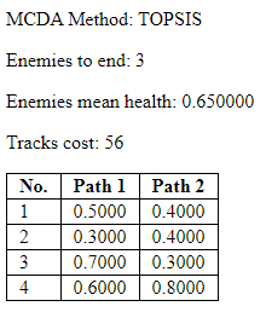
\includegraphics[width=4cm]{images/scoreRoundshtml.png}
\caption{Visualization of the generated html page}
\label{Fig:scoreRoundshtml}
\end{figure} 

Figure~\ref{Fig:scoreRounds} shows the contents of the 'scoreRounds.png' file.

\begin{figure}
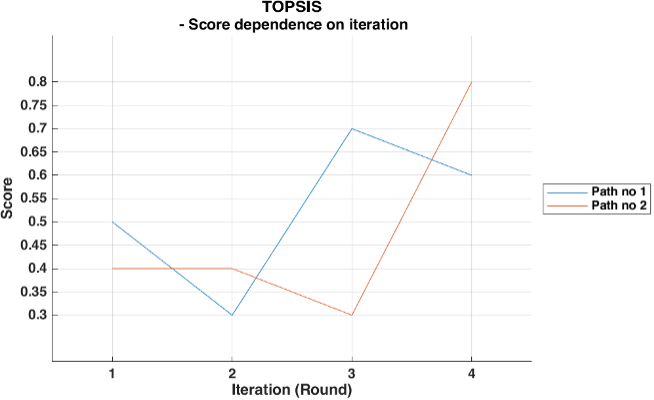
\includegraphics[width=10cm]{images/scoreRounds.png}
\caption{Contents of the 'scoreRounds.png' file}
\label{Fig:scoreRounds}
\end{figure} 

\paragraph{GenerateTabular} \hspace{0pt} \\
Generation of a tabular table.
\begin{lstlisting}[style=Matlab-editor]
GenerateTabular(fileName,data,columnDescriptions,rowDescriptions,rowsBold,decimalPlaces)
\end{lstlisting}

Description:
\begin{itemize}
\item fileName -- name of the file to which the array will be saved,
\item data -- saved array,
\item columnDescriptions -- column descriptions,
\item rowDescriptions -- row descriptions, empty array([]) means no descriptions,
\item rowsBold -- 0 means that table row descriptions are not bold, and 1 means that they are bold,
\item decimalPlaces -- number of decimal places.
\end{itemize}

Example of generating an array:
\begin{lstlisting}[style=Matlab-editor]
%Array
exampleArray = [1 2;
                  3 1;
                  5 2;
                  2 4];
%Column descriptions
columnDescriptions={'No','Date 1','Date 2'};
%Line descriptions
rowDescriptions={'1','2','3','4'};
%Creating a file containing the tabular environment
GenerateTabular('array.tex',exampleArray,columnDescriptions,rowDescriptions,0,0);
\end{lstlisting}

Contents of the array.tex file:
\lstinputlisting[style=lstStyleLaTeX]{table/array.tex}

You can attach an array to a Latex file:
\begin{lstlisting}[style=lstStyleLaTeX]
\begin{table}
\begin{tikzpicture}
\begin{axis}[
    title={Example},
    xlabel={No},
    ylabel={Data},
    legend pos=outer north east,
    ymajorgrids=true,
    grid style=dashed,
]

\addplot[
    color=blue,
    mark=square
    ]
    table[x=No,y=D1]
    {fig/array.dat};
\addplot[
    color=red,
    mark=square
    ]
    table[x=No,y=D2]
    {fig/array.dat};

    \legend{Data 1, Data 2}

\end{axis}
\end{tikzpicture}

\caption{Generated array}
\end{table}
\end{lstlisting}

The effect obtained is presented in the array~\ref{array}.

\begin{table}
\begin{tikzpicture}
\begin{axis}[
    title={Example},
    xlabel={No},
    ylabel={Data},
    legend pos=outer north east,
    ymajorgrids=true,
    grid style=dashed,
]

\addplot[
    color=blue,
    mark=square
    ]
    table[x=No,y=D1]
    {fig/array.dat};
\addplot[
    color=red,
    mark=square
    ]
    table[x=No,y=D2]
    {fig/array.dat};

    \legend{Data 1, Data 2}

\end{axis}
\end{tikzpicture}

\caption{Generated array}
\label{array}
\end{table}

\paragraph{GenerateTikzData} \hspace{0pt} \\
Generating data files for tikz charts.
\begin{lstlisting}[style=Matlab-editor]
GenerateTikzData(fileName,data,columnDescriptions)
\end{lstlisting}

Description:
\begin{itemize}
\item fileName -- name of the file to which the array will be saved,
\item data -- saved array,
\item columnDescriptions -- column descriptions.
\end{itemize}

Data generation example:
\begin{lstlisting}[style=Matlab-editor]
%Array
exampleArray = [1 2;
                  3 1;
                  5 2;
                  2 4];
%Column descriptions
column Descriptions={'No','D1','D2'};
%Creating a file containing data for tikz charts
GenerateTikzData('array.dat',[[1:size(exampleArray,1)]' exampleArray],columnDescriptions);
\end{lstlisting}

Contents of the array.dat file:
\lstinputlisting{fig/array.dat}

The array.dat file can be attached to a tikz chart:
\lstinputlisting[style=lstStyleLaTeX]{fig/array.tikz}

The effect obtained is shown in the figure~\ref{Fig:array}.

\begin{figure}
\begin{tikzpicture}
\begin{axis}[
    title={Example},
    xlabel={No},
    ylabel={Data},
    legend pos=outer north east,
    ymajorgrids=true,
    grid style=dashed,
]

\addplot[
    color=blue,
    mark=square
    ]
    table[x=No,y=D1]
    {fig/array.dat};
\addplot[
    color=red,
    mark=square
    ]
    table[x=No,y=D2]
    {fig/array.dat};

    \legend{Data 1, Data 2}

\end{axis}
\end{tikzpicture}

\caption{A chart based on data generated by the GenerateTikzData function}
\label{Fig:array}
\end{figure}

